\documentclass{article}
\usepackage[utf8]{inputenc}
\usepackage[margin = 0.8in]{geometry}
\usepackage{graphicx}
\usepackage{amsmath, amssymb}
\usepackage{subcaption}
\usepackage{multirow}
\usepackage{mathtools}
\usepackage{float}


\title{RBE502 - Homework Set 8}
\author{Keith Chester}
\date{Due date: October 27 2021}

\begin{document}
\maketitle

\section*{Introduction}

In this assignment, we will be looking at a 2 link robotic arm as depicted in the figure below. We will be designing a feedback, feedforward controller to stabilize the robotic arm on a desired orientation/position.

\begin{figure}[H]
    \centering
    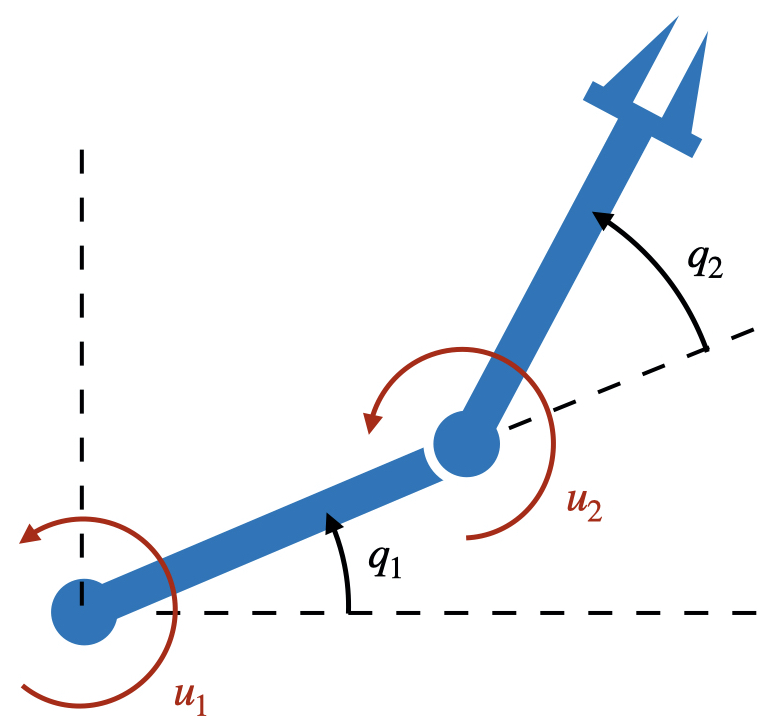
\includegraphics[width = 0.4\textwidth]{figures/2D-rr.001.jpeg}
    \caption{2 link robotic arm}
    \label{fig:robot-arm}
\end{figure}

This arm can be expressed mathematically as a double pendulum system as depicted in the following figure.

\begin{figure}
    \centering
    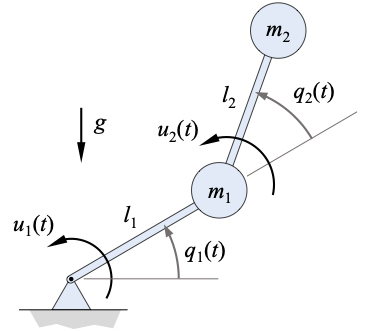
\includegraphics[width=0.4\textwidth]{figures/doublependulum.jpg}
    \caption{Double pendulum system}
    \label{fig:double-pendulum}
\end{figure}

Within this system, we can define $M(q)$, $T(q)$, and $\phi(q, \dot{q})$ as:

\begin{equation}
    M(q) = \begin{bmatrix}
        (m_1 + m_2)l_1^2+m_2*l_2^2+2l_1l_2m_2\cos{q_2} & m_2l_2(l_1\cos{q_2}+l_2) \\
        m_2l_2(l_1\cos{q_2}+l_2) & m_2l_2^2
    \end{bmatrix}
\end{equation}

\begin{equation}
    T(q) = \begin{bmatrix}1 & 0 \\ 0 & 1\end{bmatrix}
\end{equation}

\begin{equation}
    \phi(q) = \begin{bmatrix}
        (m1+m2)gl_1\cos{q_1)+m_2l_2(g\cos(q_1+q_2)-l_1\dot{q}_2(2\dot{q}_1+\dot{q}_2)\sin{q_2})}
        \\
        m_2l_2(l_1\dot{q}_1^2+g\cos{q_1+q_2})
    \end{bmatrix}
\end{equation}

We further define $x = \begin{bmatrix} q_1 & q_2 & \dot{q}_1 & \dot{q}_2 \end{bmatrix}^T$. From this we can compile these equations into a system:

\begin{equation}
    \dot{x} = \begin{bmatrix}
        q \\ \dot{q}
    \end{bmatrix} =
    f(x) + g(x)u
    =
    \begin{bmatrix}
        \dot{q} \\
        -M^{-1}\phi(q, \dot{q})
    \end{bmatrix} + 
    \begin{bmatrix}
        \boldsymbol{0} \\
        M^{-1}T(q)
    \end{bmatrix} u
\end{equation}

From this we can select a desired state, $x_d$, and define the error dynamics as:

\begin{equation}
    \dot{e} = \dot{x}_d - \dot{x} = 0 - f(x) - g(x)u = -f(x_d - e)-g(x_d-e)u
\end{equation}

We further simplify this by defining $f_e(u) = -f(x_d - e)$ and $g_e(u) = -g(x_d-e)$, thus making our final equation $\dot{e}=f_e(e)+g_e(e)u$.

\section*{Part A}

In this section, we will write $\phi(q, \dot{q})=\begin{bmatrix} \phi_1(q_1, \dot{q}_1) & \phi_2(q_2, \dot{q}_2) \end{bmatrix}^T$ as $\phi(q, \dot{q})= C(q, \dot{q})q + G(q)$. To do this, we will find the vectors $C(q, \dot{q})$ and $G(q)$.

For $C(q, \dot{q})$, we factor both $\phi_1$ and $\phi_2$ for our components $q_1$ and $q_2$. This results in the following vectors factored for each, where $\phi_{if}$ is the factored vector of $\phi_i$:

\begin{equation}
    C(q, \dot{q}) = \phi_{1f} + \phi_{2f} = \begin{bmatrix}
        -2\,l_1 \,\sin \left(q_2 \right)\\
        -l_1 \,\mathrm{\dot{q}_2}\,\sin \left(q_2 \right)
        \end{bmatrix} + \begin{bmatrix}
            l_1 \,l_2 \,m_2 \,\mathrm{\dot{q}_1}\,\sin \left(q_2 \right)\\
            0
            \end{bmatrix} = \begin{bmatrix}
                l_1 \,l_2 \,m_2 \,\mathrm{\dot{q}_1}\,\sin \left(q_2 \right)-2\,l_1 \,\sin \left(q_2 \right)\\
                -l_1 \,\mathrm{\dot{q}_2}\,\sin \left(q_2 \right)
                \end{bmatrix}
\end{equation}

To solve for G, we will first need to find the potential energy of the system, $U$, which consists of the potential energy of each link, $U_1$ and $U_2$.

\begin{equation}
    U_1 = g\,l_1 \,\sin \left(q_1 \right)\,{\left(m_1 +m_2 \right)}
\end{equation}

\begin{equation}
    U_2 = g\,m_2 \,{\left(l_2 \,\sin \left(q_1 +q_2 \right)+l_1 \,\sin \left(q_1 \right)\right)}
\end{equation}

\begin{equation}
    U = U_1 + U_2 = g\,l_1 \,\sin \left(q_1 \right)\,{\left(m_1 +m_2 \right)} + g\,m_2 \,{\left(l_2 \,\sin \left(q_1 +q_2 \right)+l_1 \,\sin \left(q_1 \right)\right)}
\end{equation}

$G(q)$ is the partial gradient of the potential energy by $q$ where $q=\begin{bmatrix} q_1 & q_2 \end{bmatrix}^T$.

\begin{equation}
    G(q) = \frac{\partial U}{\partial q} = \begin{bmatrix}
        g\,m_2 \,{\left(l_2 \,\cos \left(q_1 +q_2 \right)+l_1 \,\cos \left(q_1 \right)\right)}+g\,l_1 \,\cos \left(q_1 \right)\,{\left(m_1 +m_2 \right)}\\
        g\,l_2 \,m_2 \,\cos \left(q_1 +q_2 \right)
        \end{bmatrix}
\end{equation}

Thus our equation with a solved $C(q, \dot{q})$ and $G(q)$ is:

\begin{equation}
    \phi(q, \dot{q}) = C(q, \dot{q})\dot{q} + G(q)
\end{equation}

\begin{equation}
    \phi(q, \dot{q}) = 
    \begin{bmatrix}
        l_1 \,l_2 \,m_2 \,\mathrm{\dot{q}_1}\,\sin \left(q_2 \right)-2\,l_1 \,\sin \left(q_2 \right)\\
        -l_1 \,\mathrm{\dot{q}_2}\,\sin \left(q_2 \right)
        \end{bmatrix}
    + \begin{bmatrix}
        g\,m_2 \,{\left(l_2 \,\cos \left(q_1 +q_2 \right)+l_1 \,\cos \left(q_1 \right)\right)}+g\,l_1 \,\cos \left(q_1 \right)\,{\left(m_1 +m_2 \right)}\\
        g\,l_2 \,m_2 \,\cos \left(q_1 +q_2 \right)
        \end{bmatrix}
\end{equation}

\section*{Part B}

Here, we define values for $m_1$, $m_2$, $l_1$, $l_2$, and $g$ respectively to $10kg$, $4kg$, $1m$, $2m$, and $9.8\frac{m}{s^2}$. We are aiming to define a PD controller with gravity compensation as $u = \begin{bmatrix} K_p & K_d \end{bmatrix} (x_d-x)+G(q)$. We further define $\begin{bmatrix} K_p & K_d \end{bmatrix}$ as:

\begin{equation}
    \begin{bmatrix} K_p & K_d \end{bmatrix} = \begin{bmatrix}
        2 & 0 & 3 & 0 \\
        0 & 12 & 0 & 7
    \end{bmatrix}
\end{equation}

We aim to simulate this system from an initial position $x_0 = \begin{bmatrix}0 & 0 & 0 & 0 \end{bmatrix}^T$ to various positions.

\subsection*{$x_d = \begin{bmatrix}0 & \frac{\pi}{2} & 0 & 0 \end{bmatrix}^T$}

\begin{figure}[H]
    \centering
    \begin{subfigure}{0.325\textwidth}
        \centering
        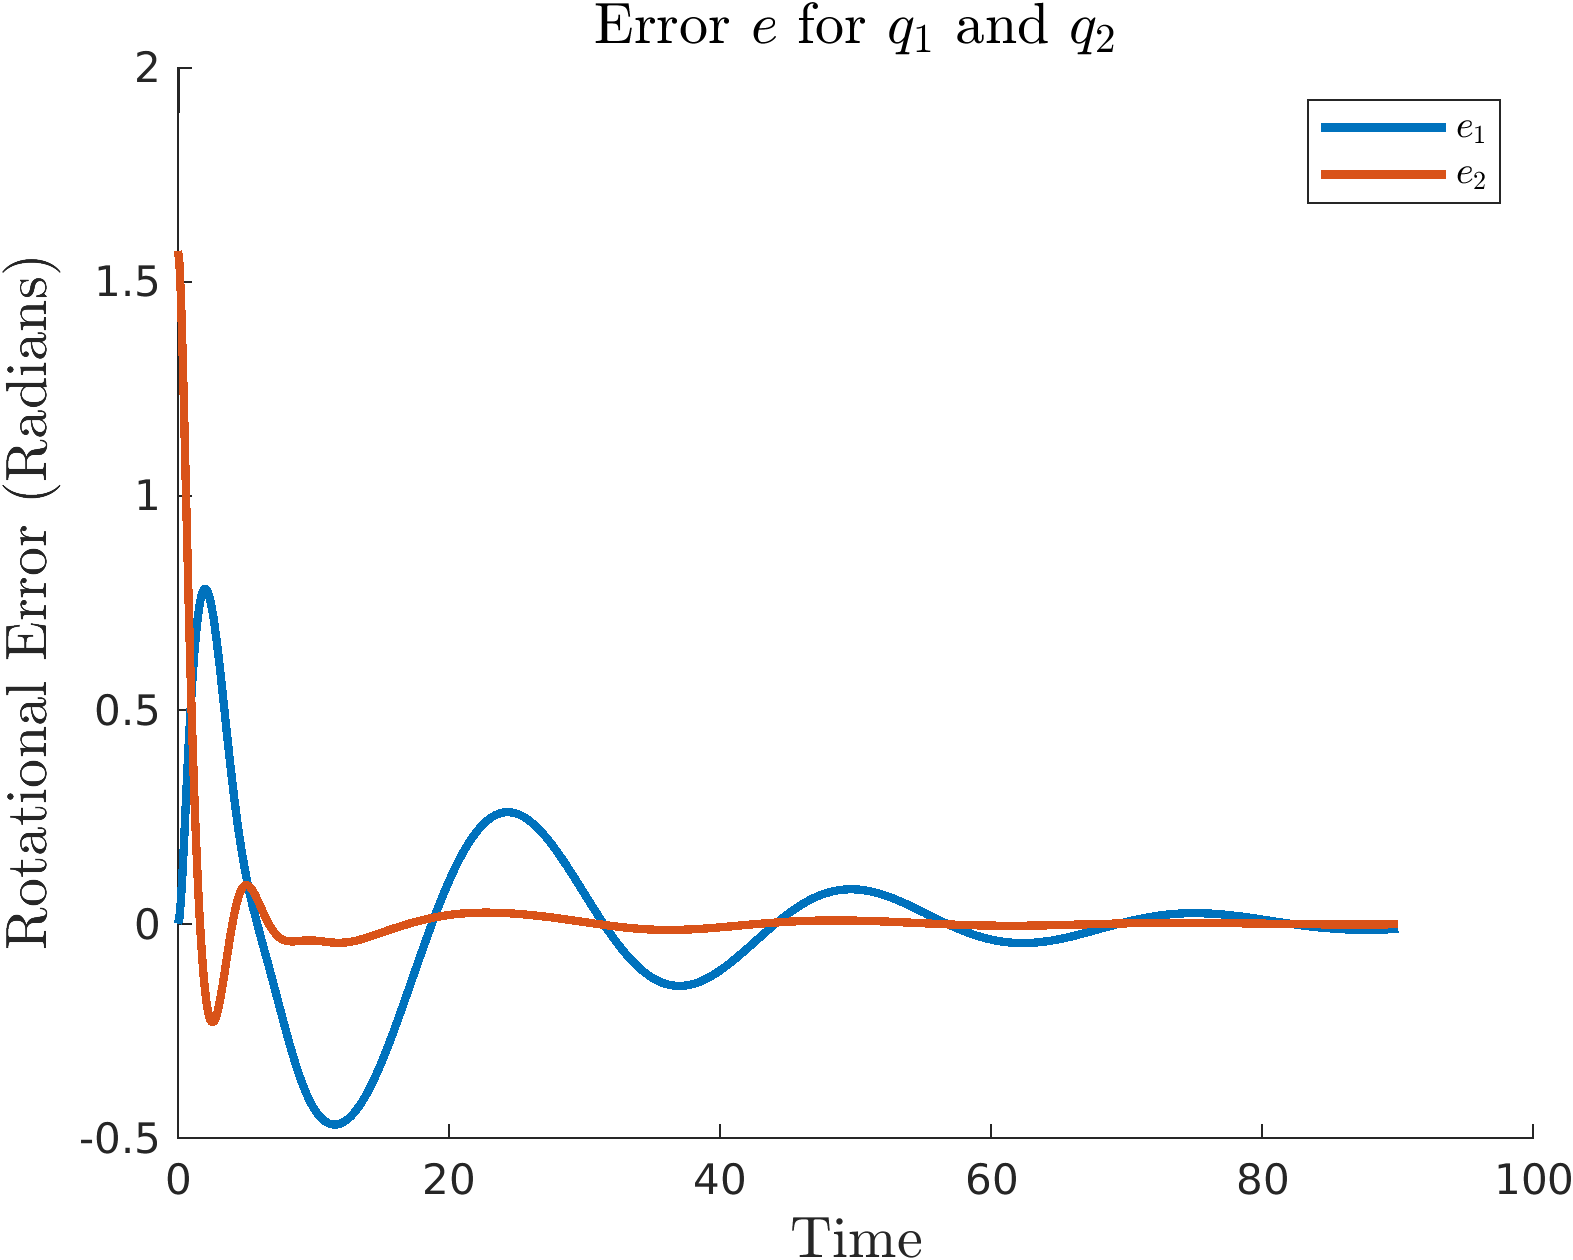
\includegraphics[width = \textwidth]{figures/error-b1.png}
        \caption{Error over time}
    \end{subfigure}
    \begin{subfigure}{0.325\textwidth}
        \centering
        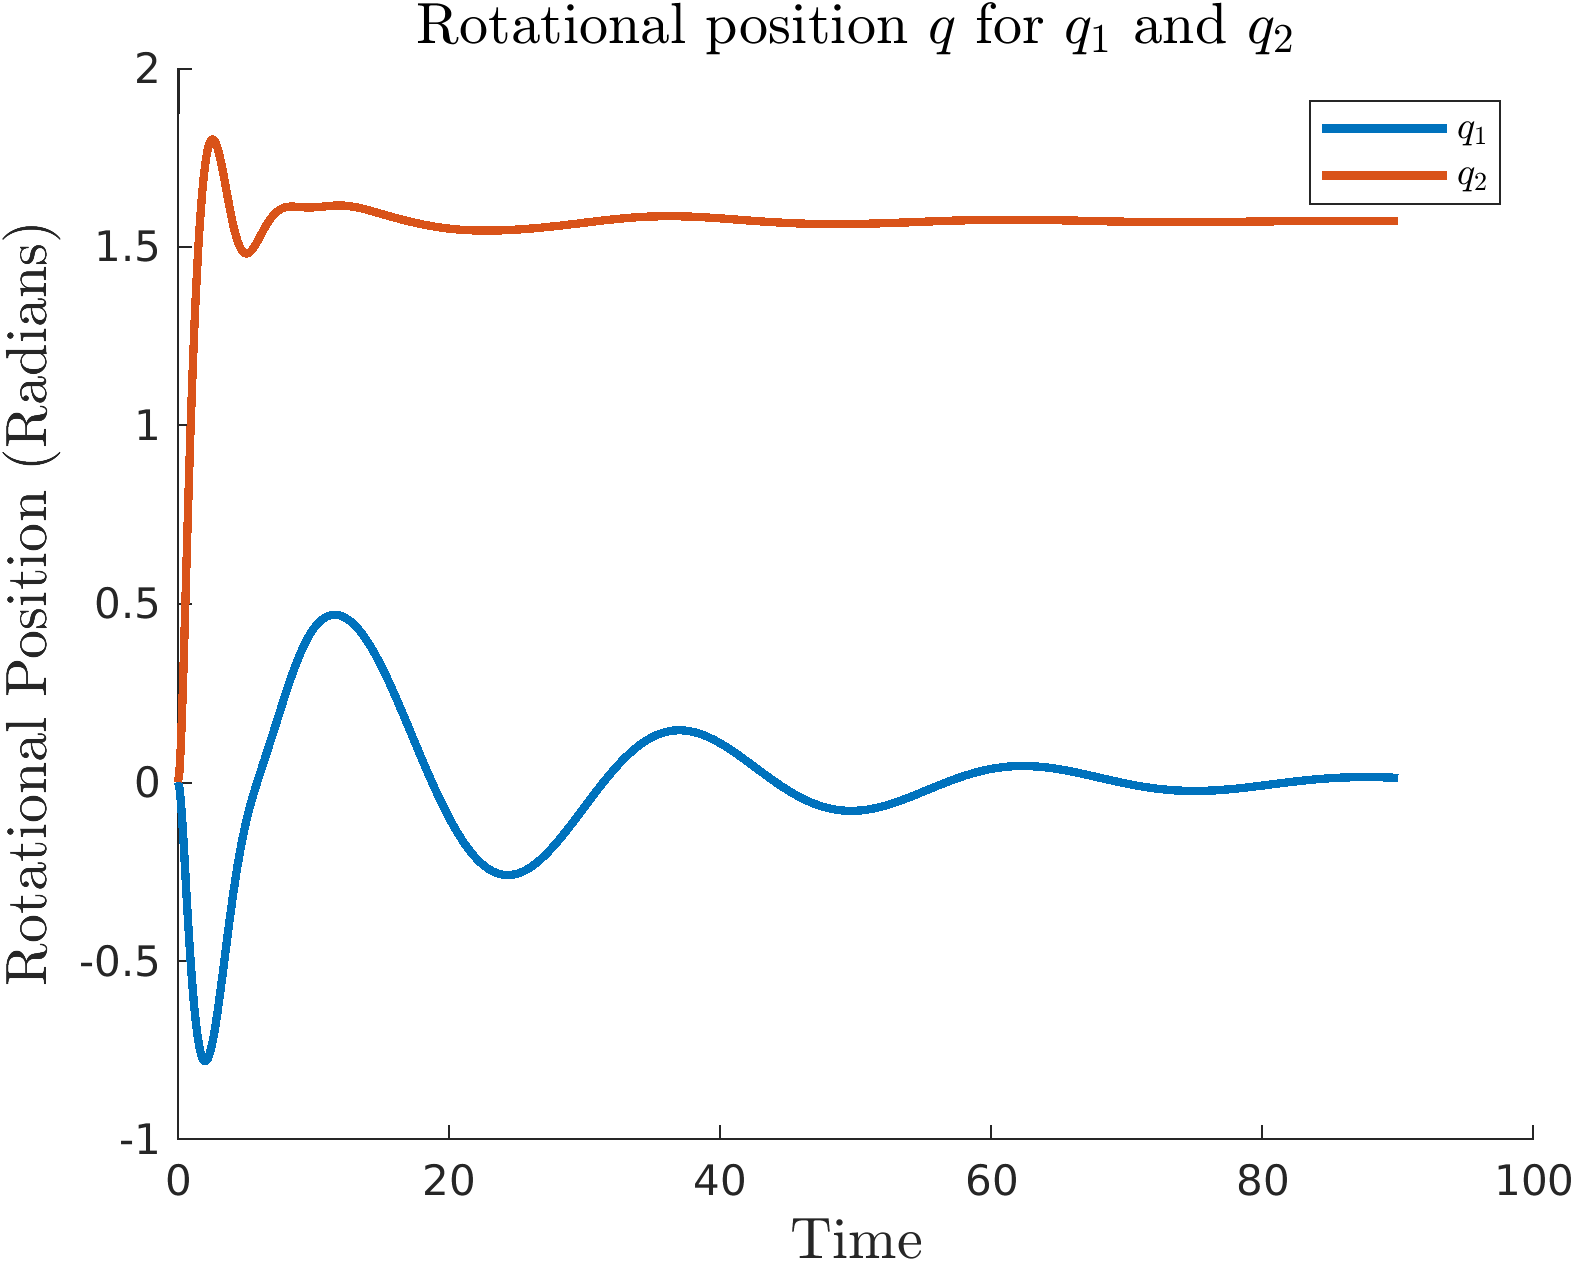
\includegraphics[width = \textwidth]{figures/rotational-position-b1.png}
        \caption{Rotational position over time}
    \end{subfigure}
    \begin{subfigure}{0.325\textwidth}
        \centering
        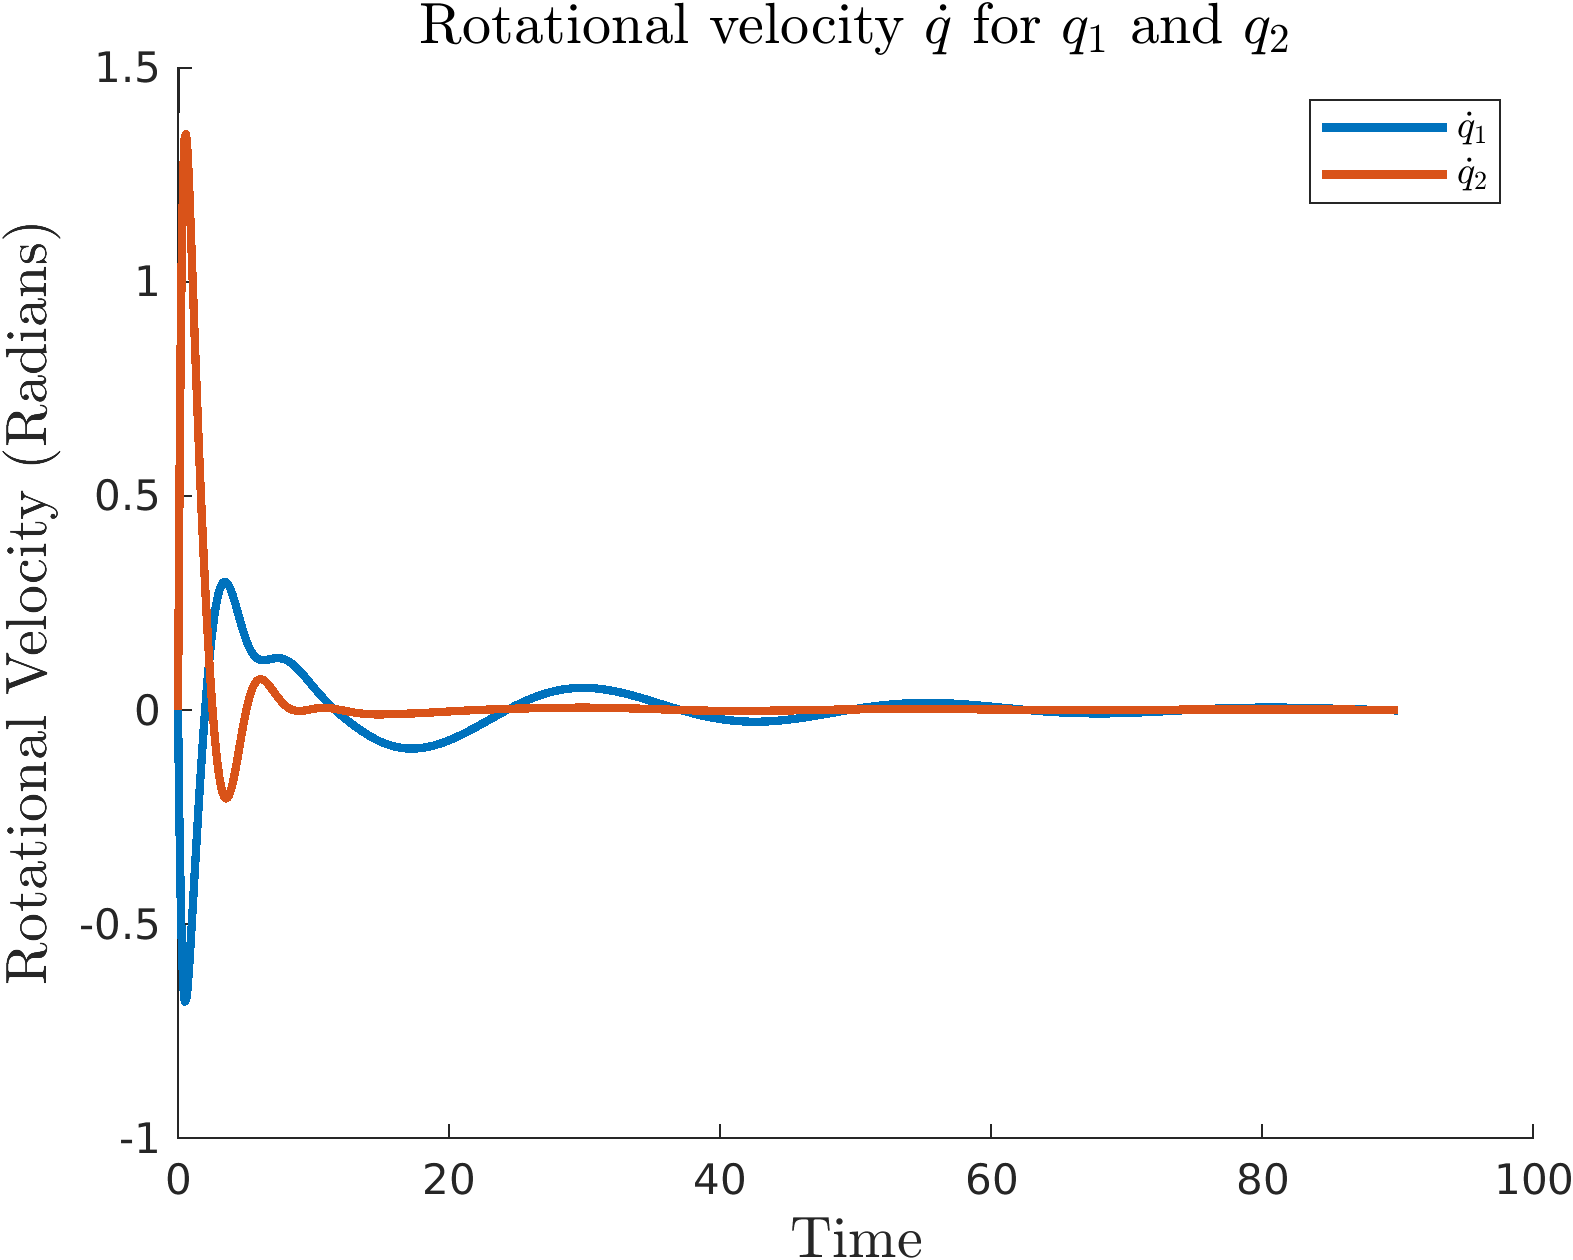
\includegraphics[width = \textwidth]{figures/rotational-velocity-b1.png}
        \caption{Rotational velocity over time}
    \end{subfigure}
    \caption{System response with $x_d=\begin{bmatrix} 0 & \frac{\pi}{2} & 0 & 0 \end{bmatrix}^T$}
    \label{fig:b-1_results}
\end{figure}

\subsection*{$x_d = \begin{bmatrix}\frac{\pi}{2} & 0 & 0 & 0 \end{bmatrix}^T$}

\begin{figure}[H]
    \centering
    \begin{subfigure}{0.325\textwidth}
        \centering
        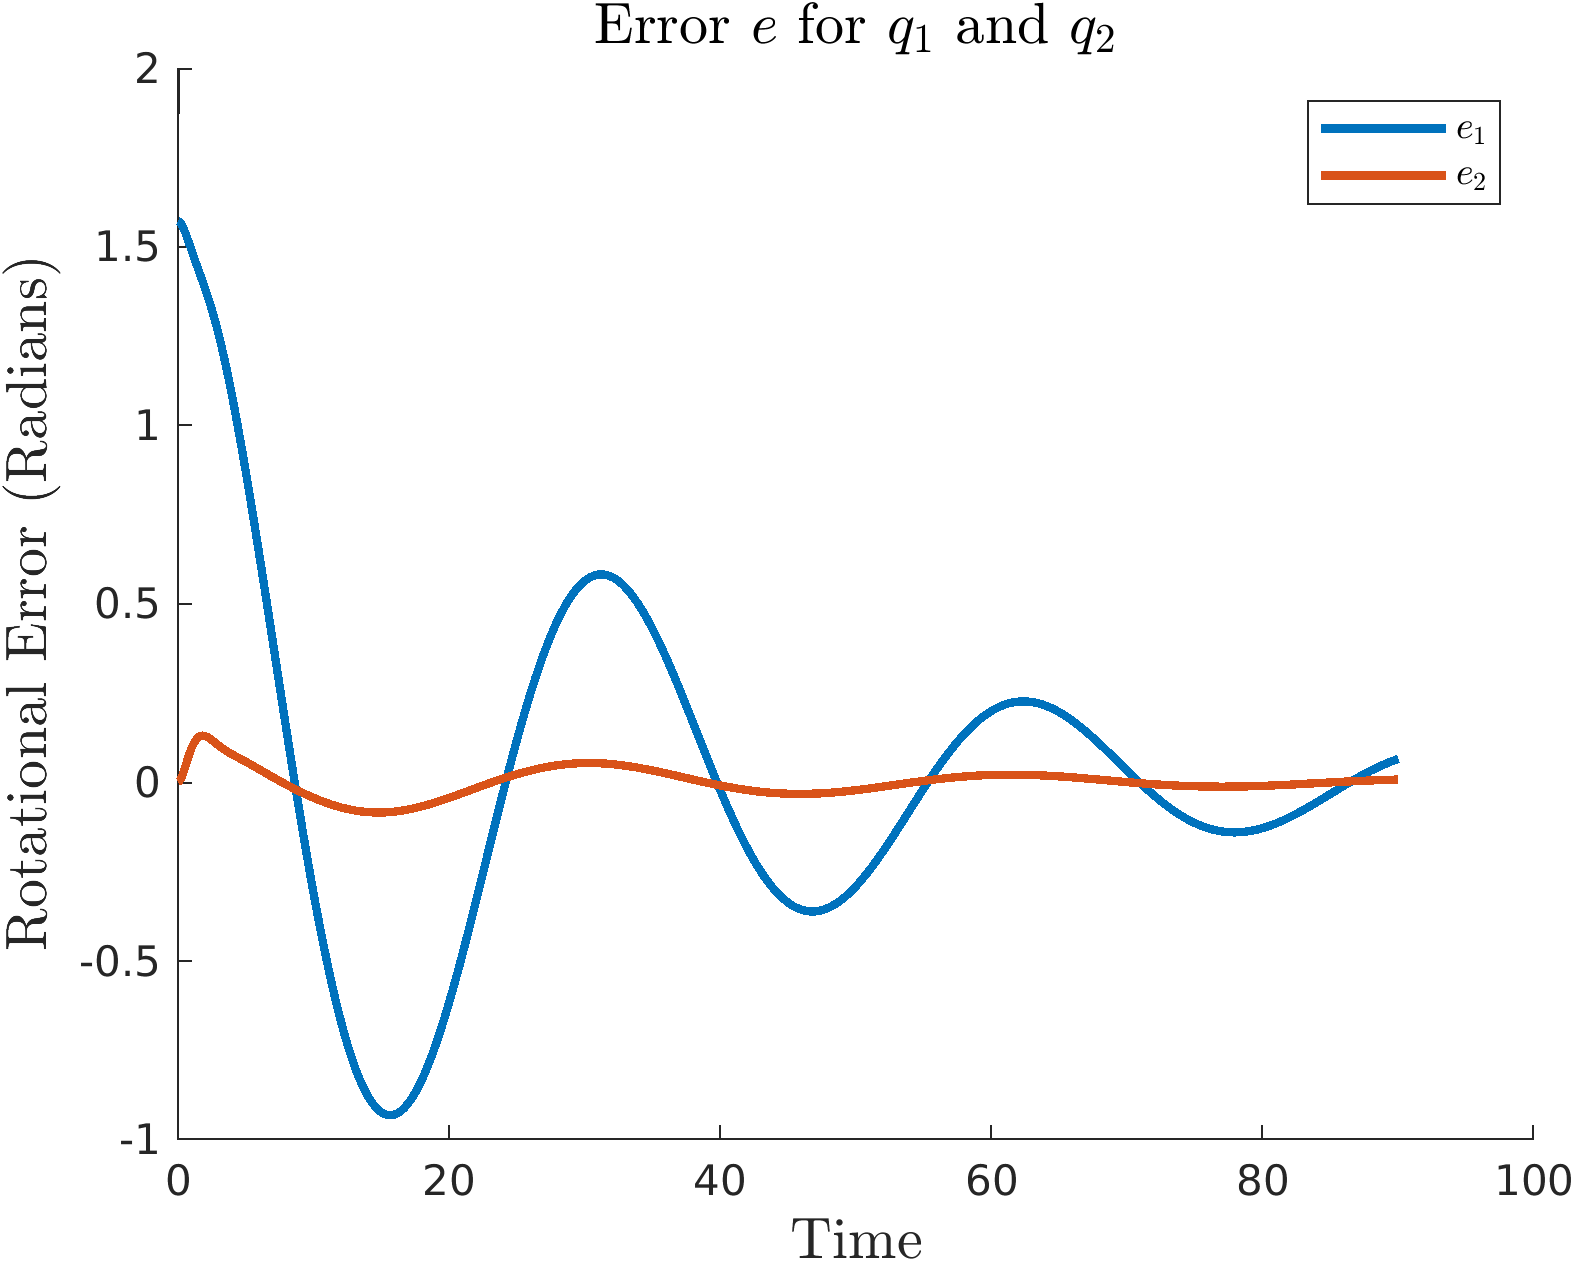
\includegraphics[width = \textwidth]{figures/error-b2.png}
        \caption{Error over time}
    \end{subfigure}
    \begin{subfigure}{0.325\textwidth}
        \centering
        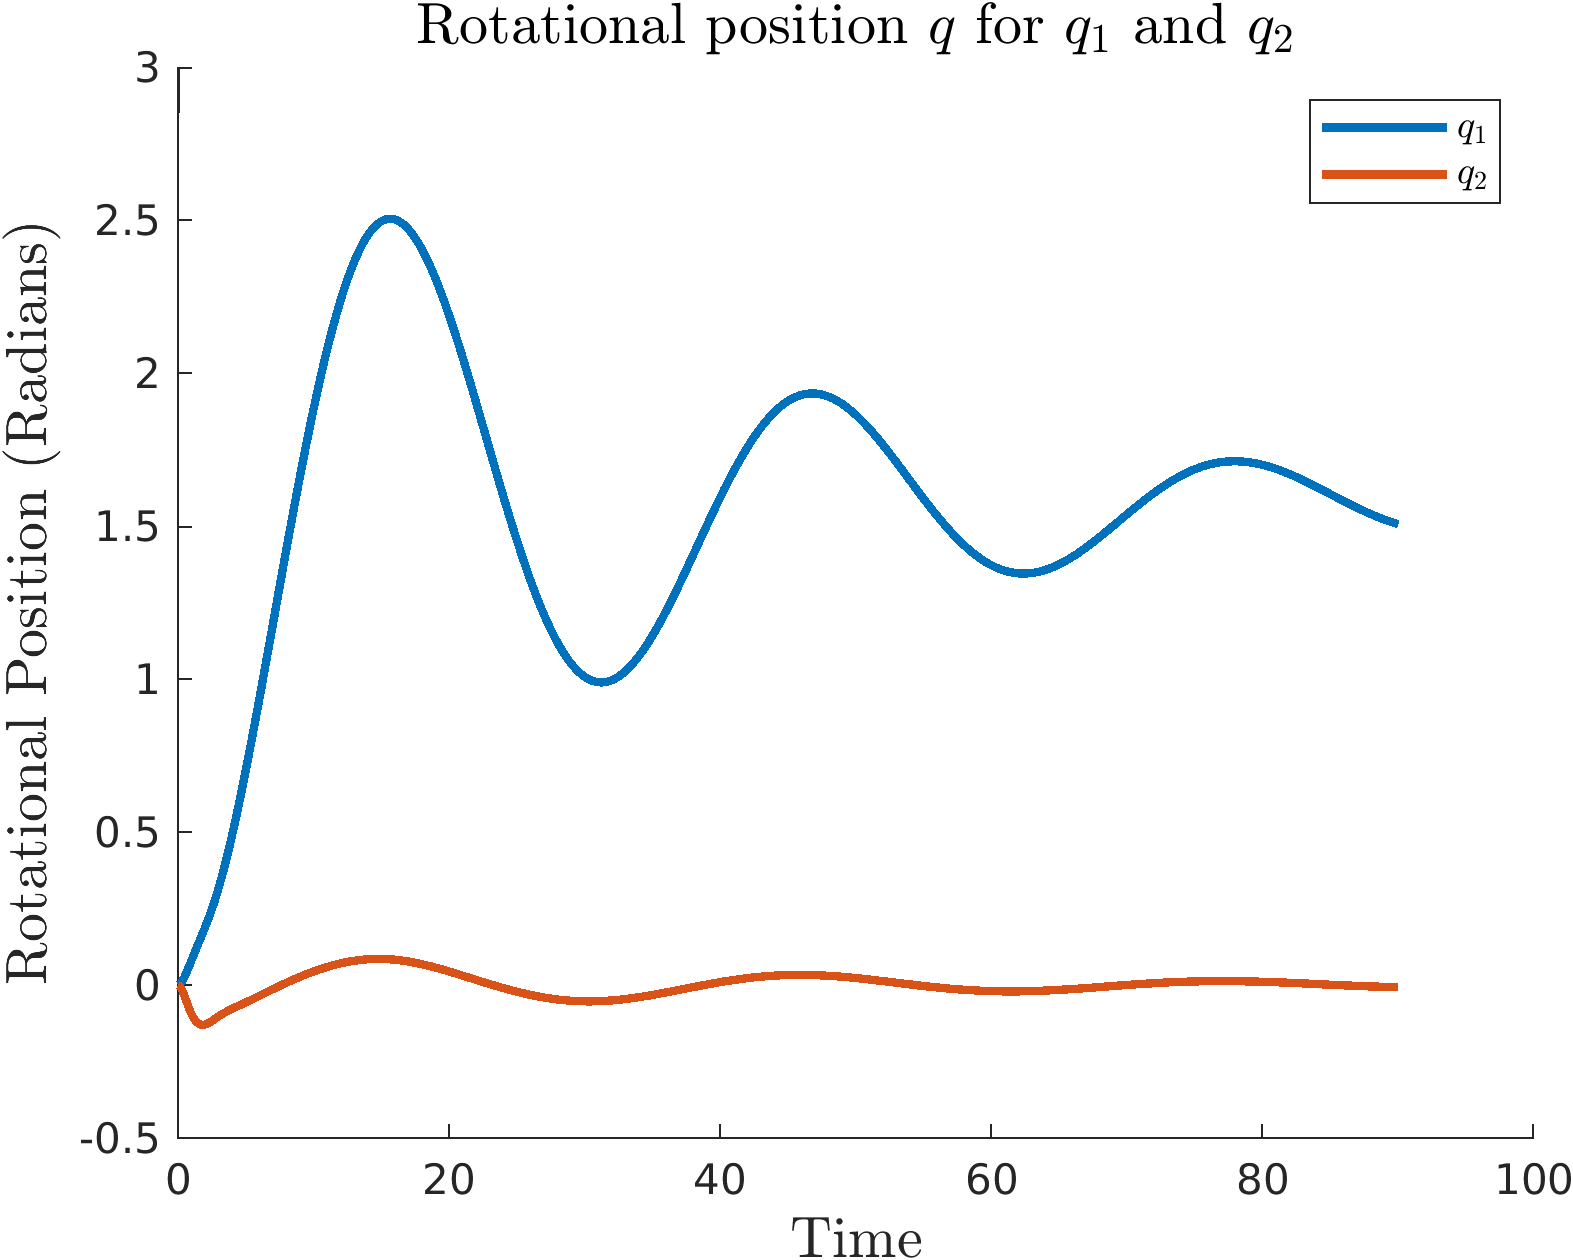
\includegraphics[width = \textwidth]{figures/rotational-position-b2.png}
        \caption{Rotational position over time}
    \end{subfigure}
    \begin{subfigure}{0.325\textwidth}
        \centering
        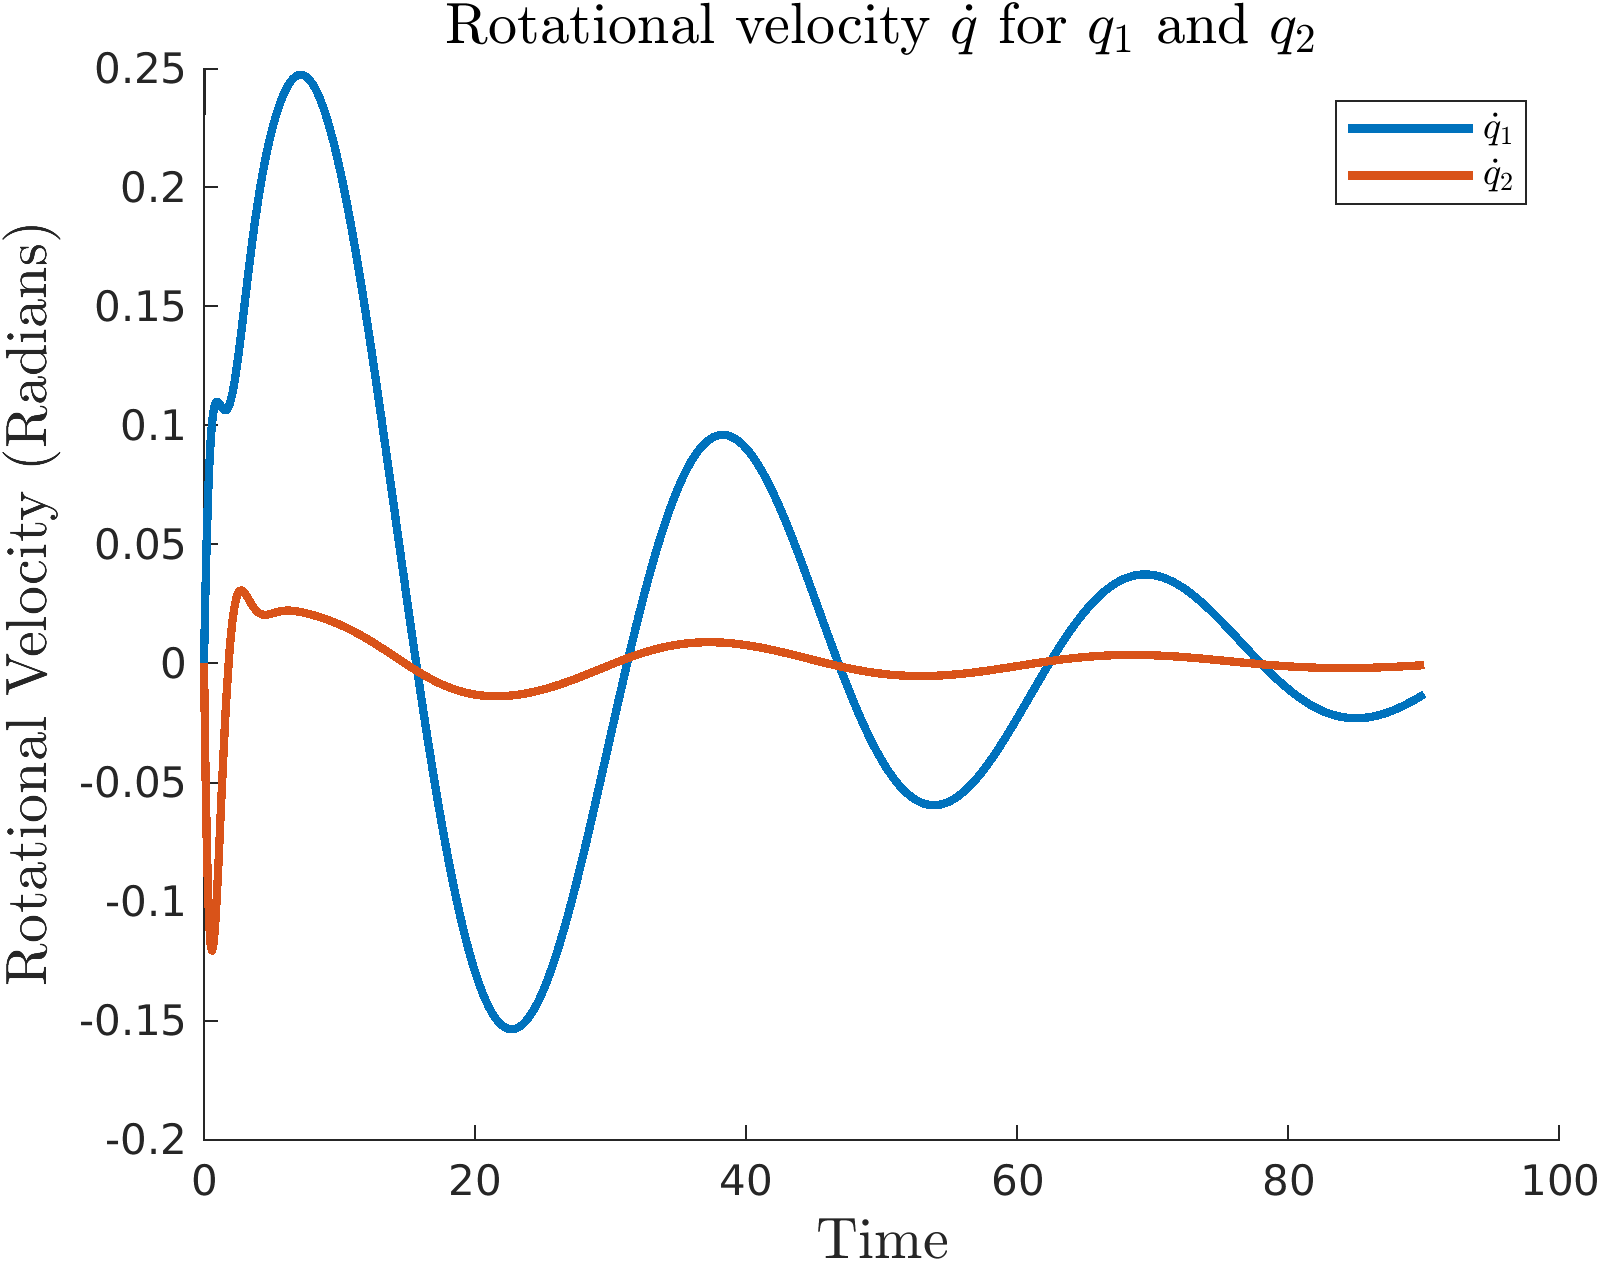
\includegraphics[width = \textwidth]{figures/rotational-velocity-b2.png}
        \caption{Rotational velocity over time}
    \end{subfigure}
    \caption{System response with $x_d=\begin{bmatrix} \frac{\pi}{2} & 0 & 0 & 0 \end{bmatrix}^T$}
    \label{fig:b-2_results}
\end{figure}

\subsection*{$x_d = \begin{bmatrix}\frac{\pi}{4} & \frac{\pi}{4} & 0 & 0 \end{bmatrix}^T$}

\begin{figure}[H]
    \centering
    \begin{subfigure}{0.325\textwidth}
        \centering
        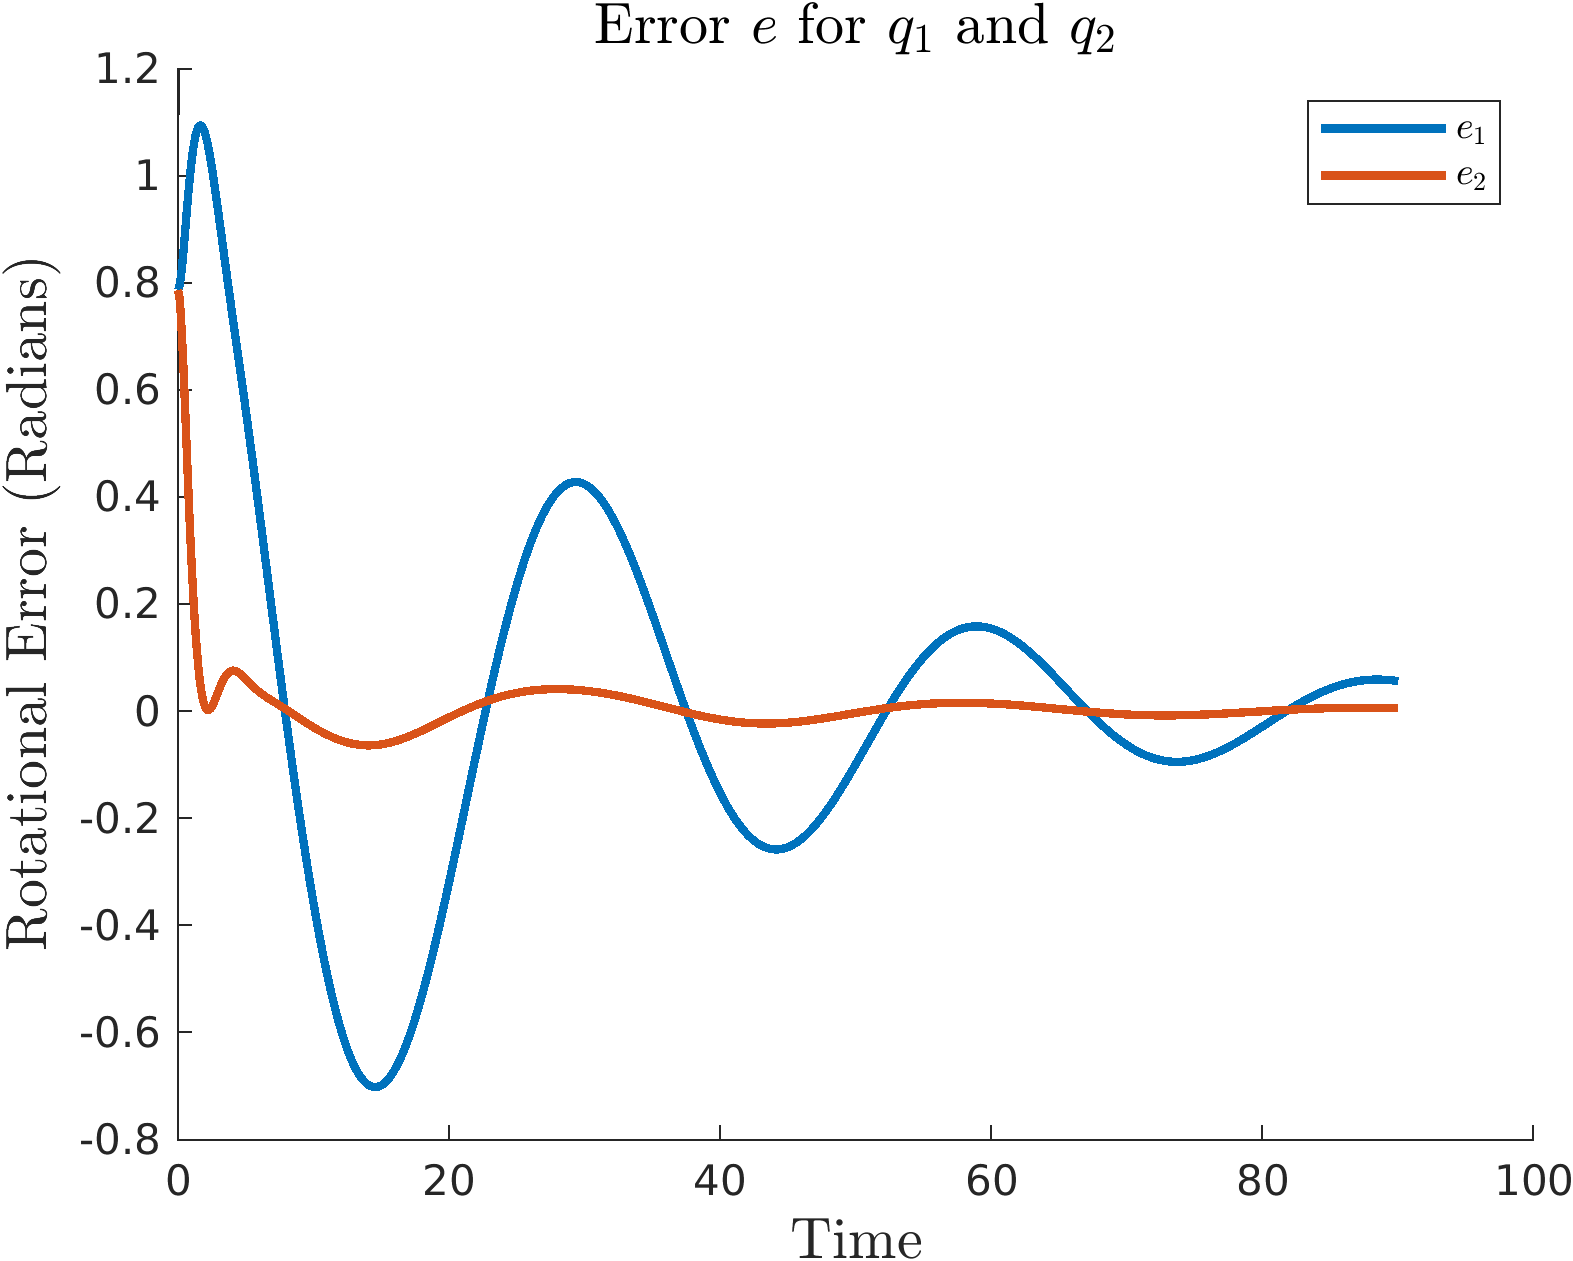
\includegraphics[width = \textwidth]{figures/error-b3.png}
        \caption{Error over time}
    \end{subfigure}
    \begin{subfigure}{0.325\textwidth}
        \centering
        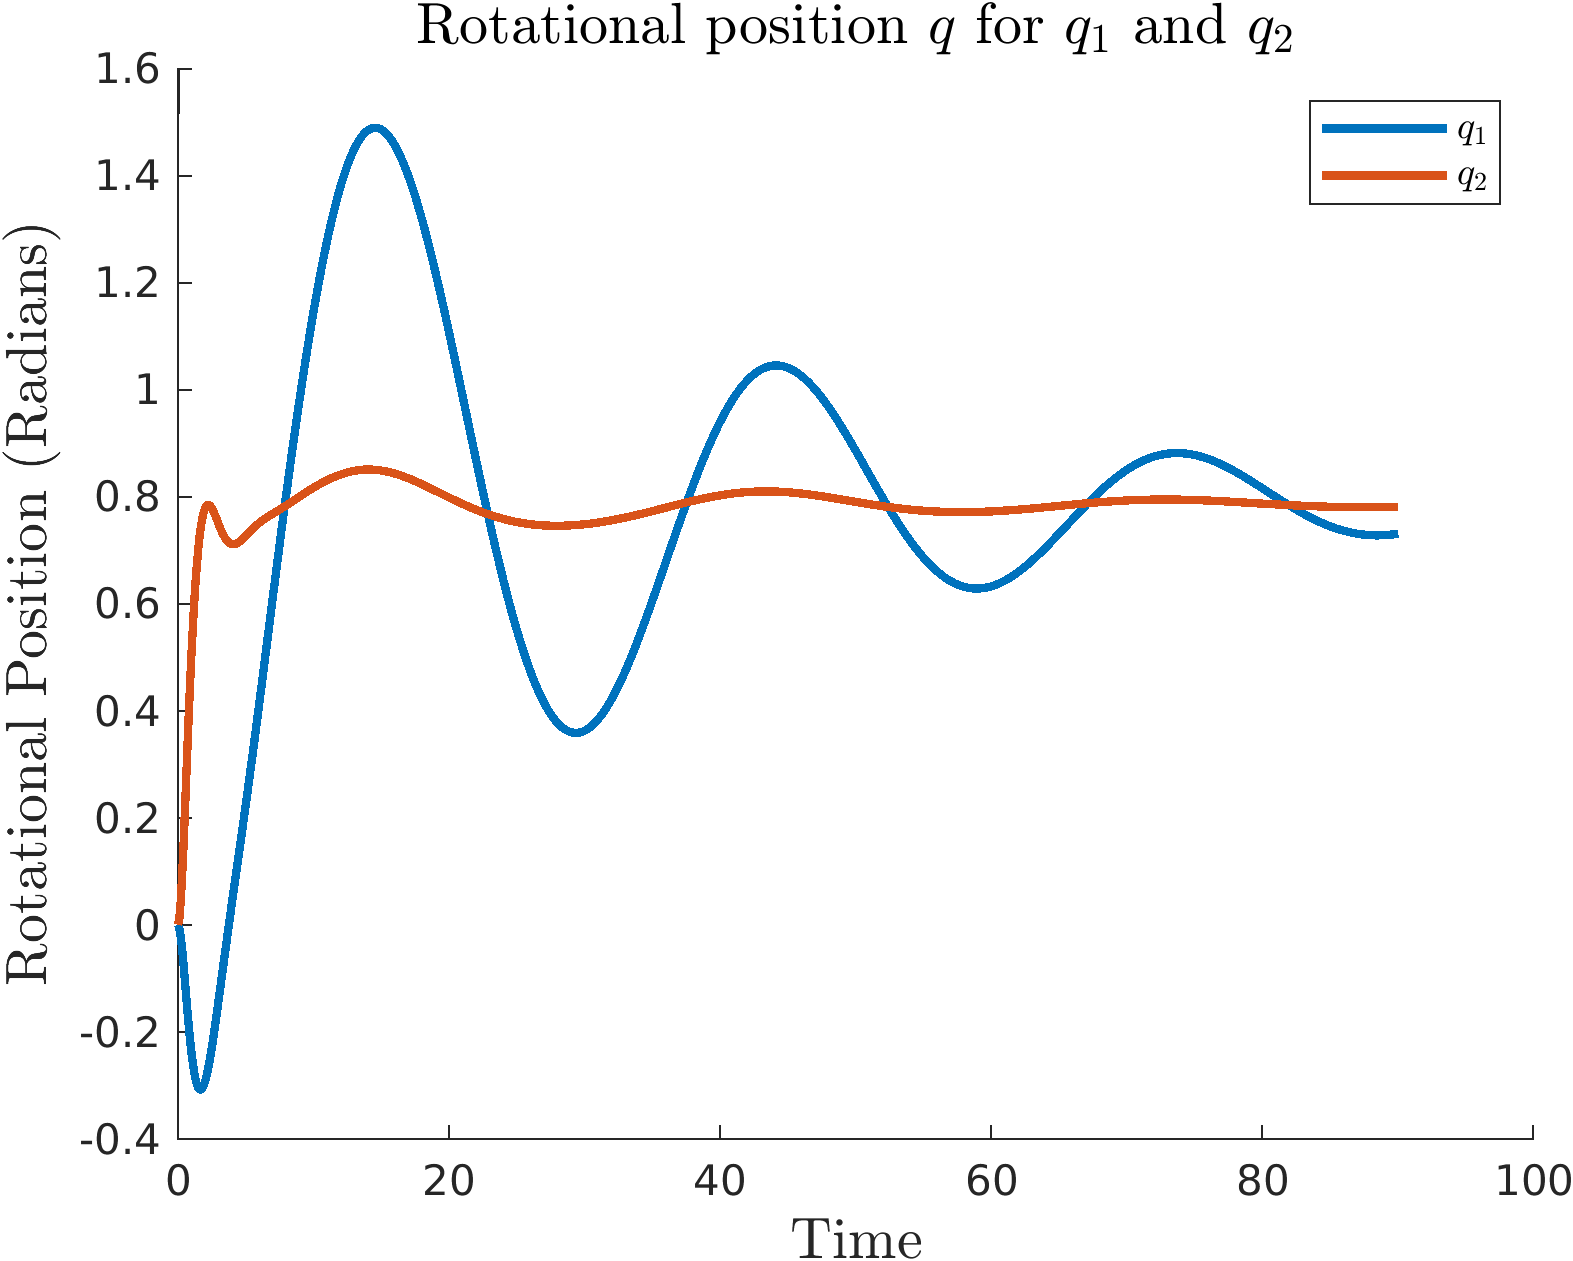
\includegraphics[width = \textwidth]{figures/rotational-position-b3.png}
        \caption{Rotational position over time}
    \end{subfigure}
    \begin{subfigure}{0.325\textwidth}
        \centering
        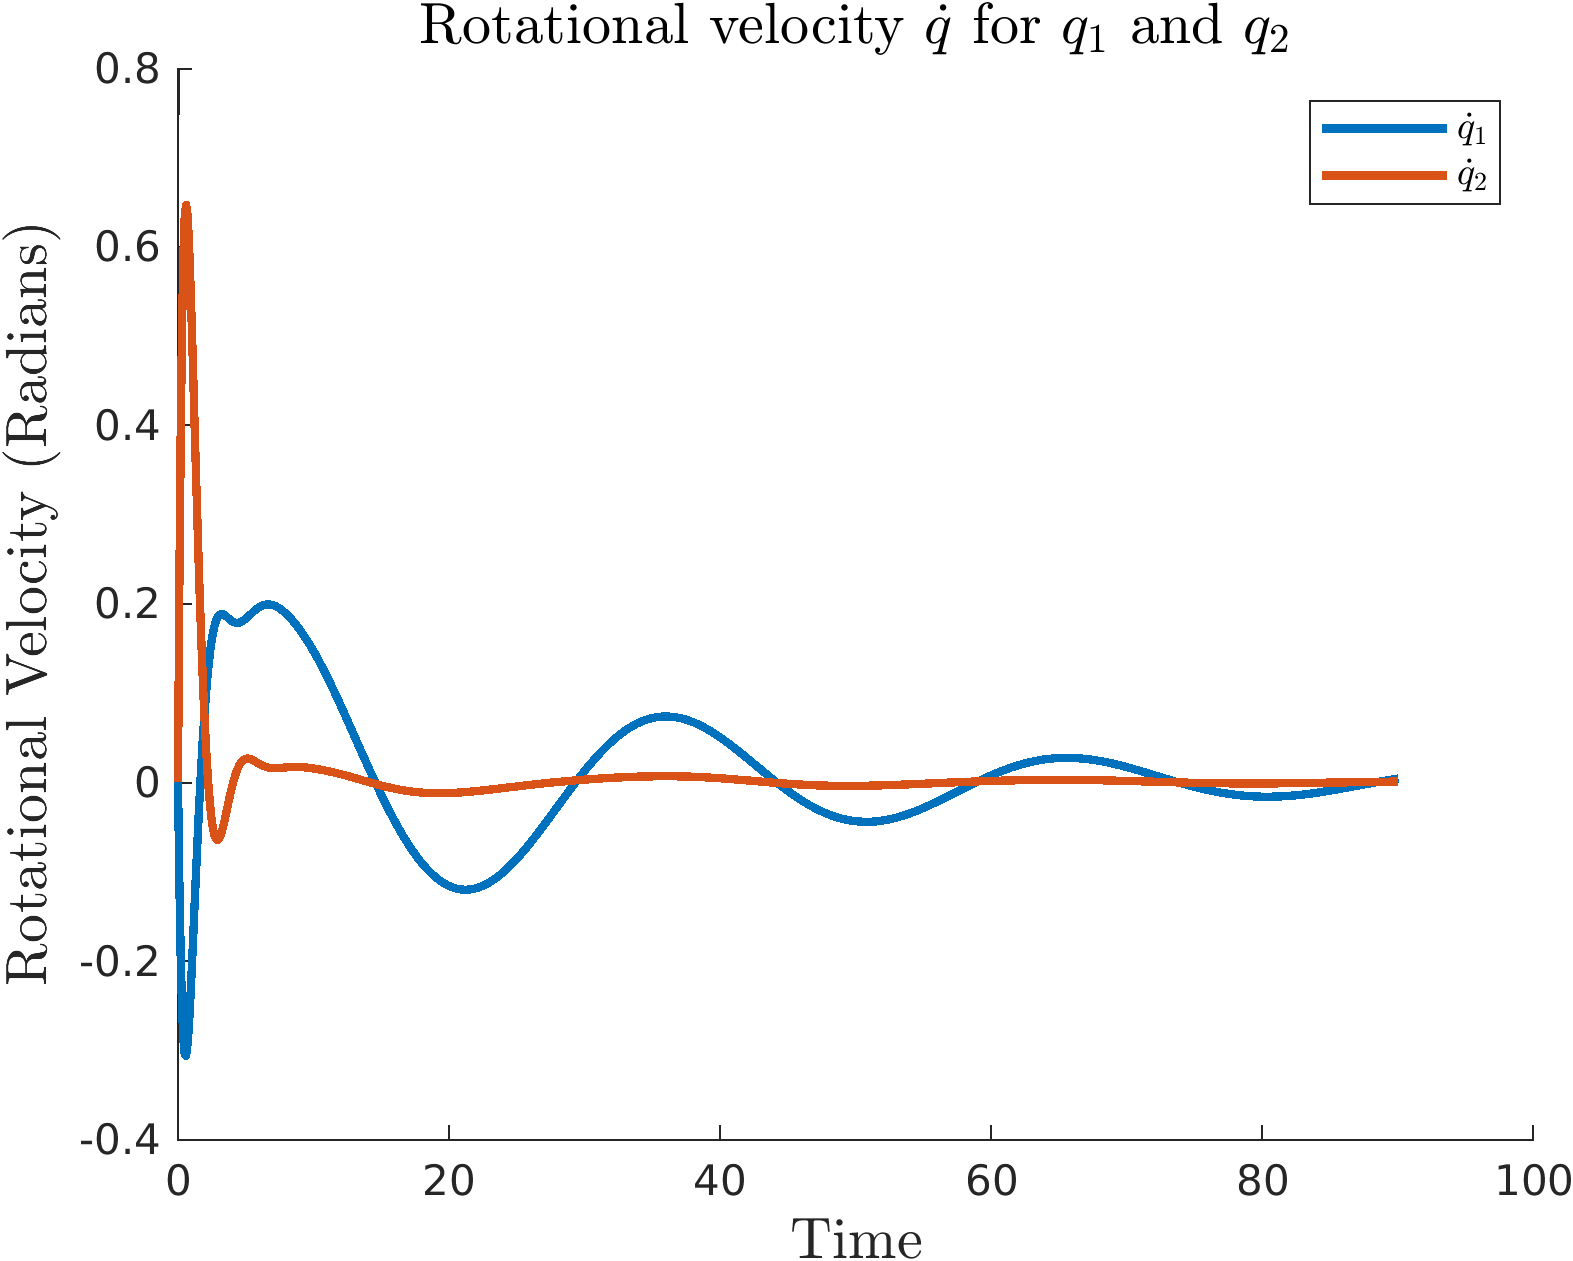
\includegraphics[width = \textwidth]{figures/rotational-velocity-b3.png}
        \caption{Rotational velocity over time}
    \end{subfigure}
    \caption{System response with $x_d=\begin{bmatrix} \frac{\pi}{4} & \frac{\pi}{4} & 0 & 0 \end{bmatrix}^T$}
    \label{fig:b-3_results}
\end{figure}

\subsection*{Part B Conclusions}

We see that these systems do converge onto a given location, but at a far slower rate than we saw with feedback lineraization. We also see that we also have significant movement of joints that were otherwise in the correct position prior.

To experiment, we modified some values in both the $K_p$ and the $K_d$ control matricies. Modifying the $K_p$ values resulted in control over the magnitude of the initial swings of error, but resulted in larger and longer oscillations. We did see faster overall convergence when tweaking the $K_d$ values to higher values, but still struggled to find a convergence time below 20 seconds.

Likewise, looking at the rotaton velocities and large changes in rotations in both joints to achieve the desired positions, this control system seems almost inefficient in its approach to establishing the desired orientation of $q_d$.

This gravity compensation is, from this experiment, better at holding a position against gravity or outside perturbances than being utilized as a methodology for moving an arm into a widely different desired orientation.

\end{document}